\section{Project execution}
Projects at the eScience Center range from 3 months to 5 years in a duration, depending on the call through which they were
granted. In all call projects, the PM (supported by Lead RSE) monitors progress and involves relevant stakeholders as needed. 
The Lead RSE takes a central role during the execution phase, ensuring regular team meetings -- typically monthly for the full team (varies with team size) 
and bi-weekly with the LA LA and/or LA team.

From a technical project management perspective, an eScience project is a research process that requires a flexible execution plan rather than a one-size-fits-all approach.
The team must adapt to unexpected challenges and deviations from initial plans, if necessary. Therefore, 
during execution phase, the Lead RSE and RSEs are encouraged to utilize diverse project management and communication methods, 
such as those mentioned in Section~\ref{sec:scope:sc}, including Turing Way~\cite{the_turing_way-2023}, minimalist project management~\cite{microp3}, the SCRUM guide~\cite{scrum-guide}, ShapeUp~\cite{agilefirst2024shapeup}, and other best practices~\cite{beck2004xp,wilson2014best}.


\subsection{Project logging}
\label{sec:exec:log}
eScience project team members routinely log important project events and agreements. The project log is placed in the
Project portfolio. The Lead RSE keeps the log up to
date (see example in Appendix~\ref{app:example-log}). The project log facilitates the information flow between
different stakeholders about project activities.

The following should be included in the project log:
\begin{itemize}[itemsep=-4pt,parsep=4pt]
\item RSD project page URL (see instructions for the RSD page in Appendix~\ref{app:rsd-page})
%\item important meetings, including dates, links to slides and fully written agreements/decisions
\item key meetings with dates, links to slides, and decisions
\item infrastructure used and decisions regarding infrastructure
%\item output/deliverables (their URLs, or this is registered as an output in RSD)
%\item participation in workshops, external events, conferences related to the project (or this is registered as an output in RSD)
\item workshop/conference participation (or this is registered as an output in RSD)
%\item changes to the project team
\item management plan updates
\item technology plan decisions and updates
\item (Code) review outcomes.
\end{itemize}

Links pointing to other documents (e.g., files in the Project portfolio, project output, repositories) should be used in
the project log to improve readability of the log and avoid duplicate information.

\subsection{Status update meetings}
\label{sec:exec:status}
The PM stays informed about the status of the project and communicates with the Lead RSE on a regular basis.

\begin{table}[h!]
\begin{booktabs}{colspec={|>{\bfseries}m{0.15\textwidth}|m{0.8\textwidth}|},row{even}={gray!20}}
    \toprule
    Scheduled: &  Once every 4-6 weeks \\[1.5ex]
    Stakeholders: & PM (organizer), Lead RSE, optionally: TL\ftnotelbl{ft:tlparticipation}, other RSEs. \\[1.5ex]
    Purpose: &  Status update on the project and discussion around project management. \\[1.5ex]
    Duration: & 30 min –- 1 hour \\[1.5ex]
    Location: & In-person meeting is default. \\[1.5ex]
    \bottomrule
\end{booktabs}
\end{table}
\ftnotetxt{ft:tlparticipation}{The TL participation is mandatory for the techology-oriented projects.}

PM and Lead RSE discuss:
\begin{itemize}
\item project status (including any changes in a project workplan)
\item technological issues, with due consultation of TL, respective SIG, or other RSEs, if necessary
\item changes in technology plan, technological choices (Section~\ref{sec:init:techplan}), management plans (Section
\ref{sec:exec:mp}). For any of these changes, TL presence is required
\item synergies with other projects in the Center
\item issues related to the budget, communication, staffing, etc.
\item knowledge development and transfer, potential for software reuse, software sustainability.
\end{itemize}

The frequency and duration of these meetings are at the discretion of the PM and depend on factors such as the
experience of the Lead RSE and the size of the team and/or the project. 

In projects that have a stronger focus on technology (such as the \href{https://doi.org/10.5281/zenodo.13829436}{eTEC}, \href{https://doi.org/10.5281/zenodo.6602816}{CIT}, \href{https://doi.org/10.5281/zenodo.10865584}{SS} projects), the TL is involved in these
meetings more frequently. For some projects, update meetings can be combined (e.g., for projects within the same Call)
or organized in the context of a larger meeting (such as a SIG on a relevant topic). Together with the Lead RSE, the PM
decides on the format of the status update meeting.


\subsection{Project team meetings}
To keep the entire project team informed on project progress, the Lead RSE together with the LA organizes a periodical
project meeting. The frequency and format depend on the complexity of the project and size of the project team.

\begin{table}[h!]
\begin{booktabs}{colspec={|>{\bfseries}m{0.15\textwidth}|m{0.8\textwidth}|},row{even}={gray!20}}
    \toprule
    Scheduled: &  Once every 2-6 weeks \\[1.5ex]
    Stakeholders: & Lead RSE or LA (organizer), LA (chair), RSEs and other project team members from the LA side. \\[1.5ex]
    Purpose: &  Progress update on the project by all team members. \\[1.5ex]
    Duration: & 30 min –- 1 hour \\[1.5ex]
    Location: & In-person meeting is default. \\[1.5ex]
    \bottomrule
\end{booktabs}
\end{table}

The agenda of this meeting should include:
\begin{itemize}
\item status update from all stakeholders
\item discussion of scientific progress
\item discussion of technological progress, issues and choices
\item alignment of project progress with the project workplan, and adjustment of the latter, if necessary.
\end{itemize}

\subsection{Writing hours and managing project budget}
\label{sec:exec:budget}
The PM and Lead RSE must have a firm grasp of the project budget and the project duration. This information is in the
Awarding letter, the proposal and Exact.

The project execution phase roughly consists of three parts: exploration, development, sustaining.
In call projects, the budget is roughly split as follows: 25\% for 
exploration (including learning), 50\% for development, and 25\% for sustaining (including research
and dissemination activities). The Lead RSE must consult the PM if project execution deviates from this plan. 
%
The left plot of Figure~\ref{fig:project-budget} assumes a constant budget spending rate. If possible, RSEs are encouraged to complete the first two phases faster, 
keeping the end date unchanged. This leaves more time for the sustaining phase (cf. Figure~\ref{fig:project-budget}), which benefits outputs like publications. 
It also leads to more effective budget use under the current eScience Center financial system.


The LA and RSEs are free to spend the awarded hours ahead of the project end date. However, the Lead RSE is responsible 
for results being delivered on time for the project and not exceeding the budget, and timely informing the PM and the LA 
about any changes to the agreed planning. If a project budget is fully spent ahead of its schedule, the PM asks Finance to restrict writing on the
project budget only to the PM.

\begin{figure*}[t!]
    \centering
    \begin{subfigure}[b]{0.49\textwidth}
        \centering
        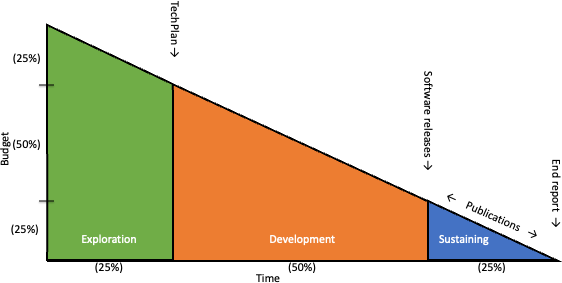
\includegraphics[width=0.97\textwidth]{img/budget-stages.png}
        \vspace{0.2cm}
        %\caption{Standard}
    \end{subfigure}%
    \hfill
    \begin{subfigure}[b]{0.49\textwidth}
        \centering
        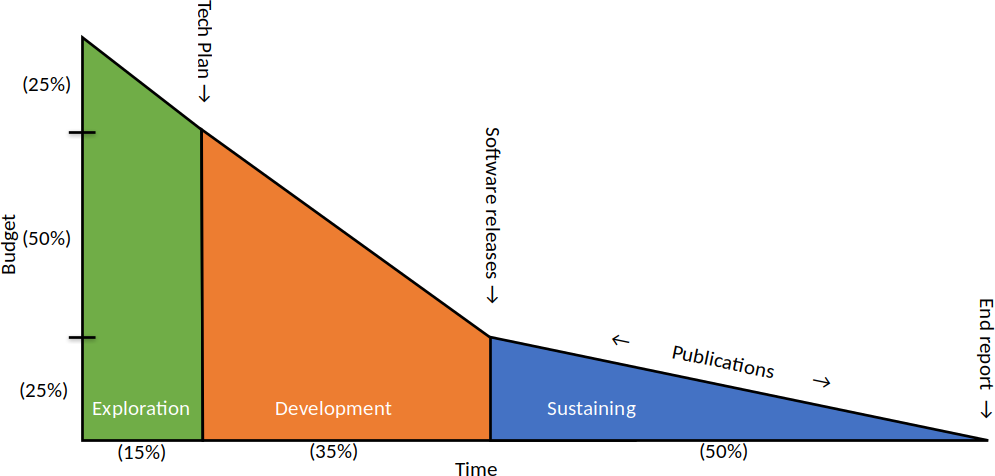
\includegraphics[width=0.97\textwidth]{img/budget-faster.png}
        \vspace{0.2cm}
        %\caption{Fast}
    \end{subfigure}
    \caption{Project's budget breakdown: standard (left) and fast (right)}
    \label{fig:project-budget}
\end{figure*}

The eScience project team (including PM and RSEs) must submit project hours in Exact by the end of each month. All entries must be completed within one working week after month-end. 
%Hours must be submitted and approved on time, preferably on a weekly basis.
%
For regular call projects, RSEs can write hours once the project is active in Exact, typically within a month of grant approval. The PM records management hours on the project budget. 
%
Project hours are managed by different parties with different responsibilities:%, see Table~\ref{tab:budget}.
\let\myhcolw\relax 
\newlength{\myhcolw}
 \setlength{\myhcolw}{0.6\textwidth}
\begin{table}[!htb]
% \caption{Parties at the eScience Center and their responsibilities}
\renewcommand{\arraystretch}{1.5}
\begin{booktabs}{colspec={|p{0.1\textwidth}|p\myhcolw|p{0.3\textwidth}|},row{even}={gray!20}}
    \toprule
    \textbf{Stakeholder} &  \textbf{Responsibilities} & \textbf{More info} \\\toprule
    PM & 
    \begin{minipage}[t]{\myhcolw}
    \begin{itemize}[itemsep=-4pt,parsep=4pt,leftmargin=0.5cm]
        \item reviews and approves project hours by the 5th workday of the following month.
        \item shares monthly hour status with RSEs via Ganttic
        \item flags issues (e.g., incorrect budgets) to Finance
        \item notifies Finance of budget changes.
    \end{itemize} 
      \end{minipage}
    & \\\midrule
    Lead RSE &     
    \begin{minipage}[t]{\myhcolw}
    \begin{itemize}[itemsep=-4pt,parsep=4pt,leftmargin=0.5cm]
        \item monitors project hour expenditure 
        \item signals deviation from the workplan to the PM
    \end{itemize} 
      \end{minipage}
    &  %Asks PM for hours status in Exact or via Ganttic  
    \\\midrule
    Finance &
    \begin{minipage}[t]{\myhcolw}
    \begin{itemize}[itemsep=-4pt,parsep=4pt,leftmargin=0.5cm]
        \item maintains accurate budget information 
        \item monitors and processes approved project hours
        \item shares monthly financial info with budget holders (PMs). 
        \item recalculates project budget if extended past year threshold.
        \item sets project to read-only if hours are depleted/exceeded early.
    \end{itemize} 
      \end{minipage}  
    & All budget changes require a formal decision (see~\ref{sec:exec:changes}). \\\midrule
    DoT & 
    \begin{minipage}[t]{\myhcolw}
    \begin{itemize}[itemsep=-4pt,parsep=4pt,leftmargin=0.5cm]
        \item monitors and approves software sustainability hours 
    \end{itemize} 
      \end{minipage}
    & There is a separate protocol on handling software sustainability. \\
    \bottomrule
\end{booktabs}
%\label{tab:budget}
\end{table}

It is possible to travel for a project, however RSEs must ask approval of their line managers (a respective SH) before
committing to an event requiring travel and fill out a travel form. See the Intranet for more information.

For \textbf{external projects}, only the PM and RSEs formally working on the project may write hours. Some projects 
(e.g., Horizon Europe) allow only direct project activities -- non-project activities like SIG involvement cannot be charged on the project. 
The Lead RSE and PM must know these restrictions or consult Finance if unsure.

\subsection{Workshops}
\label{sec:exec:workshops}

Some call projects require the LA to organize workshops. These workshops aim at fostering research communities around
the software developed in projects. Workshops may focus on early user feedback, new features, or connecting existing tools to broader communities. 
%
Based on the call text, the PM and Lead RSE determine whether one of more workshops must be organized. 
Finance provides the project's workshop budget status. There are two types of workshops, namely, (a) organised by the LA, and (b) organized by the Lorentz Center.
%
\paragraph{For workshops organized by the LA:} the LA writes and submits the workshop plan(s) to Finance in a timely manner 
(see~\cite{proj-portfolio} for templates). Finance approves the plans in consultation with the PD and PM. 
The Lead RSE is expected to contribute to the workshop and its organization. A CM can advise the LA (through the Lead RSE) on
fostering engagement and growth of relevant software communities; a CM is involved in the introductory
part of the workshop, including addressing attendees. Finance handles the administrative and financial aspects of the 
request and requests feedback on the scientific content from the PM team.


%Detailed procedure of workshops approval is described in Appendix~\ref{app:workshops}.
%
\paragraph{For workshops organised by the Lorentz Center:} the LA must apply through the Lorentz Center webpage.
%\footnote{The procedure is described in the eScience - Lorentz Center Agreement and Annexes {\textcolor{red}(add the link when signed)}.}.
%
The LA has the leading role in the application. The Lead RSE takes an advisory role in the writing and design of the
workshop proposal and is expected to actively participate during the workshop event. The PM must ensure enough hours
are allocated for the Lead RSE (or RSE from the project team) to help the LA with the proposal and attend the workshop,
if they want to take an active role.

These workshops differ from the eScience-Lorentz Center Competition workshops that are jointly funded by the eScience and
the Lorentz Center. Besides co-funding expenses, the eScience Center provides an additional in-kind support. 
The role of the eScience RSEs is described in the awarded proposals. The project
initiation and the eScience team assignment follow the usual process. The team
collaborates with the organizers on planning and outcome of the workshop (e.g. research paper, white paper, software
release, or grant consortia). The Lead RSE plays a pivotal role in preparing and
delivering the workshop, and, possibly, in publishing any outcome drafted during the event. 

\subsection{Data and Software Management Plans}
\label{sec:exec:mp}
For some projects, Data and Software Management Plans (DMP~\cite{dmp-guide} and SMP~\cite{smp-guide}) outline how project data and software are maintained. 
%
Depending on the call, the LA must submit complete DMP and SMP documents within 6 months of the project. The Lead RSE 
may assist in drafting the DMP, which the LA submits to the PM, who asks a TL for review and approval. For call projects since 2021, SMPs are included in project proposals.

The LA is responsible for keeping both plans up to date and must inform the PM and TL of changes via the Lead RSE. The PM may request updates as needed, with support from the Lead RSE.


\subsection{Knowledge transfer}

To increase visibility of the project and its results, the project team (including RSEs, PM, TL), Communications, CMs,
share knowledge and outcomes both inside and outside of the organization. The Lead RSE ensures that
\begin{itemize}
\item project results are timely shared with Communications, CMs, and relevant SH;
\item project and software pages on the RSD are properly updated; and
\item specific requests to facilitate project visibility are sent to Communications by RSEs.
\end{itemize}

Moreover, PMs, Lead RSEs and TLs work together to spot opportunities for cross project collaboration (e.g., by reusing
software or knowledge in these projects or as a new reusability project, read more in Section~\ref{sec:opportunities:ss}).



\subsubsection{Output management}
\label{sec:exec:output}
Project deliverables include research articles, presentations, talks, posters, tutorials, datasets, blog posts, white papers, and workshops, 
as well as software-related outputs such as code releases, software papers, demos, videos, tutorials, and training materials. 
%
RSEs strive to apply FAIR principles~\cite{fair-principles,FAIR4RS} to all project deliverables. They should have
\begin{itemize}\itemsep0em
\item (concept) DOIs from publishers or open-access archives like Zenodo, arXiv, or DANS;
\item acknowledge the eScience Center project grant~\footnote{By adding the following sentence into the publication: "<full project title> is a project of the Netherlands eScience Center, funded under grant number <grantid>."}; and
\item listed RSEs working on the project as (co-)authors.
\end{itemize}

RSEs must record all project outputs in relevant systems and databases (see Table~\ref{tblr:output}) to ensure knowledge transfer. 
The PM expects the team to follow the deliverables plan outlined in the proposal and workplan. RSEs contribute to publications and software/data releases.

\begin{longtblr}[
  theme = fancy,
  caption = {Output management},
  %entry = {Short Caption},
  label = {tblr:output},
%  note{a} = {It is the first footnote.},
%  note{$\dag$} = {It is the second long long long long long long footnote.},
  %remark{Note} = {Some general note. Some general note. Some general note.},
  %remark{Source} = {Made up by myself. Made up by myself. Made up by myself.}
]{
 % colspec = {|X|X|X|X|X|}, width = 1\linewidth,
  colspec={|p{0.12\textwidth}|p{0.12\textwidth}|p{0.35\textwidth}|p{0.1\textwidth}|p{0.2\textwidth}|}, width = 1\linewidth,
  rowhead = 1, %rowfoot = 1,
  row{1} = {font=\bfseries},
  column{1} = {font=\bfseries},
  row{odd} = {white}, row{even} = {white},
  row{1} = {gray!20}, %row{Z} = {nlesc-yellow},
  %cell{2}{1,4,5} = {r=2}{t},
  cell{2}{1,4,5} = {r=2}{t},
  cell{4}{1,4,5} = {r=2}{t},
  cell{6}{1,4,5} = {r=3}{t},
  %cell{9}{1,4} = {r=2}{t},
}
\toprule
What & Responsibility of & Responsible for  & URL & Additional info \\
\toprule
Zenodo (NLeSC community) & PM / CMs  & curating and approving new publications & \href{https://zenodo.org/communities/nlesc/}{Zenodo link} & 
    \begin{minipage}[t]{1\linewidth}
    \begin{itemize}\itemsep0em
        \item Publications on Zenodo are added to the community
    \end{itemize} 
    \end{minipage}  \\
%\midrule
\cmidrule{2-3}
    & RSEs & getting a (concept) DOI for a data or software release, or a document (e.g., non-peer-reviewed publications) 
&  & \\
\midrule
RSD, software and project pages & PM / Lead RSE & 
    \begin{minipage}[t]{1\linewidth}
    %\vspace{-1cm}
    \begin{itemize}\itemsep0em
      \item ensure the eScience team has maintainer access 
      \item decide on reuse of the project page if the project continues under new funding.
    \end{itemize} 
    \end{minipage}  & 
    See~\cite{rsd:manual} &
  %Each project has its RSD project page. The Lead RSE in agreement with the PM can use the same RSD project if a direct continuation of the project is granted from another funding source. In this case, the funding source and respective text should be added. \\
  See Appendix~\ref{app:rsd-page}\\
\cmidrule{2-3}
    & RSEs &  
    \begin{minipage}[t]{1\linewidth}
    \begin{itemize}\itemsep0em
      \item create project page, if needed 
      \item maintain pages with complete, up-to-date metadata
    \end{itemize} 
    \end{minipage} &  & \\
\midrule
     Project portfolio & PM & adding a direct link to the project portfolio in Ganttic & 
     cf.~\cite{proj-portfolio} for structure explanation. &  
    An internal archive with regular automatic backups. Direct link to the portfolio folder available in Ganttic   \\
\midrule
    & Lead RSE & ensuring that all docs are available & & \\
\midrule
    & RSE & 
   \begin{minipage}[t]{1\linewidth}
    \begin{itemize}\itemsep0em
        \item upload outputs (e.g., papers, reports, presentations)
        \item link the source material in the project log
    \end{itemize} 
    \end{minipage} & &  \\
\midrule
%\pagebreak
  The eScience Center blog  & RSEs &  
  \begin{minipage}[t]{1\linewidth}
    \begin{itemize}\itemsep0em
        \item Create a blog post about the project, its progress, or outcomes.
        \item add final blog URL to project RSD page
    \end{itemize} 
    \end{minipage} &
  Indexed at \href{https://blog.esciencecenter.nl/}{eScience Blog} & Instructions on blogging are posted on the Intranet~\cite{intranet}
 \\
\midrule
      & Editorial Team & 
    \begin{minipage}[t]{1\linewidth}
    \begin{itemize}\itemsep0em
        \item Review blog post entry of project team 
        \item Help at any stage with writing and publishing process
    \end{itemize} 
    \end{minipage} & &   \\ 
% Foot    & &  &Foot  & Foot    \\
\bottomrule
\end{longtblr}


Open access publications and open source software are mandatory for all call projects. The PM and Lead RSE inform the LA if needed. 
Open access fees are budgeted by Finance annually in the call budget (with the PD approval); if no budget is available, alternatives can be explored:

\begin{itemize}\itemsep0em
  \item publishing through the LA's institution (either open access funds are available or the LA organization is connected to publish open access in a lot of journals through the library without a fee)
  \item choosing the best option for open-access publishing (is it a diamond or gold open-access journal)
  \item publishing closed access and self-archiving either a preprint or publication after six months under Taverne agreement in Dutch copyright law (cf.~\cite{taverne,taverne:ou}).
\end{itemize}
The Lead RSE and PM consult Finance regarding payments for an open access publication.

For \textbf{external projects} the expected deliverables are also part of the formal project documents (proposal,
contract, etc. The Lead RSE is expected to keep the PM informed of the status of deliverables throughout the project.


\subsubsection{Outreach}
\label{sec:exec:outreach}
The Lead RSE promotes the project's visibility through project demonstrators, presentations, and
other means. All RSEs are expected to communicate externally about the project and its deliverables, as
outlined in Section~\ref{sec:exec:output}. Communications supports the project team by 
highlighting project through various channels, including but not limited to news items, social media
posts, videos and interviews about relevant the scientific impact of the research software developed 
or used. The Lead RSE (or occasionally the PM) provides Communications with relevant information. 


Blog posts are an optional but highly recommended output of the projects. Any team member, from LA to RSE, can author them. 
Topics may include simplified research summaries, tutorials on learned skills or technologies, or updates on workshops, publications, and other project outputs.

RSEs share project progress and results (e.g., technology plan, milestones, code releases) with colleagues, 
including SIG presentations. Each RSE prepares and updates a 3-slide deck or pitch \cite{proj-portfolio}. 
The Lead RSE ensures a demonstrator is available after the first major software release.


The LA and their team are encouraged to participate in relevant Digital Skills Workshops~\cite{digital-skills} from the eScience Center. Furthermore, if the LA and their team
require a project-specific training workshop, the Lead RSE involves
\begin{itemize}
\item workshop coordination with CMs, who can advise on organization and training material development; Finance handles any related payments if applicable;
\item the PM discusses RSE hours spent on training organization and consults Finance if needed.
\end{itemize}

For \textbf{external projects}, consortium agreements (e.g., Non-Disclosure Agreement or NDA) may define result communication. The Lead RSE and PM review these at project start to clarify communication boundaries.

\subsection{Code quality and sustainability checks}
Ensuring software quality and sustainability is integral to the code development process cycle at the eScience
Center. All RSEs are expected to follow our software development guide and best practices~\cite{guide-nlesc}. Code should be 
designed to be as generic and reusable as possible from the start.

\subsubsection{Code development}
\label{sec:exec:code}
At the initial stage of code development in the project, the Lead RSE together with RSEs:

\begin{itemize}\itemsep0em
\item set up a GitHub organization for the project, following the eScience Center Guide and the Turing Way~\cite{the_turing_way-2023}
\item add the URL of this organization to the RSD project page.
\end{itemize}

RSEs must always ask at least one project team member, relevant SIG member or other RSE at the eScience Center to
review, comment and approve pull requests in the project codebase.

\subsubsection{Code review}
As part of the annual review (see Section~\ref{sec:exec:annual}), a code review is organized by the Lead RSE. Depending
on the project it could take the form of a reusabilithon\footnote{Coined by the Software Sustainability SIG, the term refers to a 2-3 hour session where a group of RSEs evaluates a piece of software for usability, provides feedback to the developers, and formulates recommendations to improve its (re)usability.}, a review of code on GitHub, or
something else entirely (format to be approved by TL). The reviewers for this process are typically other RSEs at the
eScience Center.


The goal is to review software of the project for:
\begin{itemize}\itemsep0em
\item its usability (reproducing steps of installations, and running it on a machine/laptop)
\item overall software quality and suitability
\item whenever appropriate, correctness of code
\item adherence to the technology plan (Section~\ref{sec:init:techplan})
\item adherence to eScience Center best practices
\item opportunities for reuse of software in other projects
\item correct inclusion in output systems (Section~\ref{sec:exec:output}).
\end{itemize}

Reviewers make written suggestions for improvements, and flag major issues encountered. These issues serve as input for
the TL for the formal annual review meeting (see Section~\ref{sec:exec:annual}). These notes are stored in the project log. 

\subsection{Annual project review meeting}
\label{sec:exec:annual}

\let\myhcolw\relax % let \myhcolw to \relax to be reused later
\newlength{\myhcolw}
\setlength{\myhcolw}{0.75\textwidth}

\begin{table}[h!]
\begin{booktabs}{colspec={|>{\bfseries}m{0.2\textwidth}|m{\myhcolw}|},row{even}={gray!20}}
    \toprule
    Scheduled: &  Yearly \\[1.5ex]
    Stakeholders: & PM (organizer, chair), Lead RSE, LA, TL, optional: other project team members, SH \\[1.5ex]
    Purpose: &  %
    \begin{minipage}[t]{\myhcolw}
    \begin{itemize}[leftmargin=0.3cm]\itemsep0em
        \item to ensure that the project is still on track
        \item to discuss any persistent issues to ensure optimal collaboration between project team
        \item to explore opportunities beyond the project  
    \end{itemize} 
      \end{minipage}
    \\[1.5ex]
    Outcomes/Actions: & List of agreed actions and PM/TL advice for next steps. \\[1.5ex]
    Duration: &  Max 1.5 hours \\[1.5ex]
    Location: &  At the eScience Center or the project location\ftnotelbl{ft:participants} \\[1.5ex]
    \bottomrule
\end{booktabs}
\end{table}
%\footnotetext[2]{Mandatory participants of a meeting be present in-person at the office, while all optional participants can also participate via video conferencing if they prefer.}


For call projects longer than one year, the PM organizes annual reviews. The details are described in the
terms and conditions document~\cite{nlesc-terms}. For one-year projects, review meetings are optional and decided by the PM in consultation with the TL and Lead RSE.

Each review includes discussion and actions on reusability and sustainability of project results (as described in the DMP and SMP), status of collaboration, and follow-up opportunities. 
%
\iffalse
The goals of the meeting are to:
\begin{itemize}
\item review progress against the original workplan
\item discuss research results, their novelty and current deliverables
\item update management plans if needed
\item plan strategies to share results with a wider community
\item address software reuse and sustainability
\item identify bottlenecks and improvements for team efficiency
\item report project budget (RSE hours remaining)
\item explore further collaboration, funding, and cross-project opportunities
\end{itemize}
\fi
The agenda of this meeting is:
\begin{itemize}\itemsep0em
\item introduction and purpose of meeting
%\item project overview and deliverables
%\begin{itemize}
\item scientific goals status (the LA and team)
\item project output status (the project team)
%\end{itemize}
\item collaboration status (including hours admin and bottlenecks)
\item use of digital infrastructure and SURF support (if applicable)
\item next steps and future opportunities.
\end{itemize}
For \textbf{external projects}, review meetings are typically part of the project process. The PM, with the Lead RSE, decides if a (lightweight) internal review is needed.


\subsubsection{Review meeting preparation}
\begin{table}[h!]
  \renewcommand{\arraystretch}{1.5}
\begin{booktabs}{colspec={|>{\bfseries}m{0.3\textwidth}|m{0.6\textwidth}|},row{even}={gray!20}}
    \toprule
     &  \textbf{Stakeholder} \\[1.5ex]\toprule
    Prepared by: & LA and Lead RSE, with optional input from other stakeholders. \\[1.5ex]
    Reviewed by: &  PM accountable for project, TL accountable for technology. \\[1.5ex]
    Target audience: & PMs, TLs, SHs and RSEs. \\[1.5ex]
    \bottomrule
\end{booktabs}
\end{table}

The Lead RSE coordinates preparations for the review meeting:
\begin{itemize}\itemsep0em
\item request the PM to share the standard review meeting slide template~\cite{proj-portfolio} with the LA team
\item requests project team members to contribute to the review meeting slides, wherever appropriate,
\item compiles technology status report (see Section~\ref{sec:exec:tech}).
\end{itemize}


LA and Lead RSE jointly prepare the slides:
\begin{itemize}\itemsep0em
\item 3-5 slides summarizing progress toward research goals. The LA is not expected to present published content or the
original workplan or proposal. If applicable, the LA reports on workshops.
\item 1-2 slides on the technology plan status, including reuse, adoption, and sustainability, supporting the technology status report.
\item highlight any scientific or technical bottlenecks and assess if the project is on track or needs replanning;
\item the PM reports on the RSE hour status (i.e. the number of hours already spent); and
\item the project team provides a feedback on collaboration and suggest improvements if needed.
\end{itemize}
 
Additionally, the Lead RSE:
\begin{itemize}\itemsep0em
\item together with the LA, ensures all output is properly registered (see Section~\ref{sec:exec:output}), and adds missing URLs/DOIs to the slides;
\item coordinates with the team to finalize the presentation at least 2 working days before the review meeting;
\item uploads the slides to the project portfolio; and
\item informs PM and TL that slides are ready and are in the project portfolio.
\end{itemize}

\subsubsection{Technology status report}
\label{sec:exec:tech}
Prior to the annual review meeting, the PM asks Lead RSE to fill in the technology status report. This report 
summarizes the technical progress of the project and includes RSD project page with its deliverables, URLs
to project plans, software quality and community involvement. The Lead RSE prepares it in collaboration with the project team; it serves as input for the TL during the review.

The Lead RSE:
\begin{itemize}\itemsep0em
\item collects output and relevant information from LA and team
\item meets with CM (for the community outreach activities) to draft the technology status report  
\item draft the rest of the report with the TL
\end{itemize}

Two weeks prior to the review meeting, the Lead RSE submits the completed report to the TL. The TL conducts a code 
review or software health check based on the report and shares the results with the eScience team. If needed, 
the Lead RSE, TL, and PM may meet to discuss the findings before the annual review meeting.

The report and the review(s) are archived by the TL in the project portfolio.

\subsubsection{At the review meeting}
The time breakdown of the meeting agenda is follows:
\begin{itemize}\itemsep0em
\item presentation by the LA (max. 20 min)
\item presentation by the Lead RSE (max. 20 min), including the RSE roles and deliverables
\item discussion (max. 40 min)
\item summary, action points and conclusions.
\end{itemize}

The PM chairs the meeting and, with the TL, acts as reviewer. The TL highlights tech/software issues. Everyone contributes to the discussion. PM and TL assess deliverables, and comment on their status:
\begin{itemize}\itemsep0em
\item have the objectives outlined in the proposal been sufficiently addressed? (PM)
\item does the project follow the workplan in terms of deliverables? (PM)
\item has the output been registered according to the rules of output management (Section~\ref{sec:exec:output})? (PM, TL)
\item does all project output have publications (including software and data papers)? (PM)
\item are there any issues flagged during the code review that needs to be discussed with the project team? (TL)
\item does the project team sufficiently engage and align with relevant communities (e.g., via the workshops)? (PM)
\item does the project adhere to the technology plan, SMP and DMP? (TL)
\end{itemize}

The eScience project team comments on any further possibilities for reusability, adoptability and sustainability of the
software, and the project team comments on possible collaborations beyond the project.

The PM updates the slides with action points, agreements and plans (with the project partners agreement). The PM logs
the meeting in the project log.

\subsubsection{After the review meeting}
PM shares the updated slide deck with the project team members to check the agreements written down. PM ensures that the
final version of the presentation(s) uploaded to the project portfolio is correct.

\subsection{Reporting}
\label{sec:exec:report}
For call projects the annual review meeting and end report (Section~\ref{sec:closing}) serve as formal progress reports.

\textbf{External projects} may require periodic reporting to the consortium on progress and deliverables. 
The PM and Lead RSE consult the agreements, contract, and workplan; Finance handles financial input. 
The external coordinator (e.g., EU project coordinator, NWO programme officer) signals deadlines on the report delivery. 
The Lead RSE drafts the eScience Center's contribution, the PM reviews it. Finance fills in the financial part of the report 
(signed by the DoO if needed). The PM submits the final report to the external project coordinator 
(via EU portal done by Finance) and archives it in the project portfolio.

\subsection{Conflict resolution and complaint procedure}
The eScience Center adheres to the Code of Conduct outlined in the Personnel Policy (cf.~\cite{cao}). 
%
Conflicts involving eScience and the LA team on the projects should be addressed using this four-step process:
\begin{enumerate}\itemsep0em
\item The Lead RSE first seeks resolution with the LA; the PM may be consulted or join in discussion if needed.
\item If unresolved, the issue is escalated to the PM (via the Lead RSE), who organizes a meeting to mediate.
\item Persistent issues can be escalated to the PD via a written summary submitted through the PM.
\item The PD may escalate to the DT if necessary.
\end{enumerate}

If the issue concerns the PM, RSEs may escalate to their manager (SH). An external confidential advisor ('Vertrouwenspersoon') is also available for anonymous support~\cite{intranet}. 
Conflict resolution may lead to project adjustments, such as staffing changes (cf. Section~\ref{sec:init:vacancy}).

\subsection{Non-RSE Consultants}
\label{sec:exec:consult}
Certain issues require consultation beyond the project team. Team members must inform the PM, who may delegate actions as needed:

\begin{itemize}\itemsep0em
\item GDPR/personal data: consult the GDPR contact~\cite{intranet}. 
\item Software/data quality and access: contact the TL.
\item Scientific integrity: contact the integrity officer~\cite{intranet}.
\item SURF-related matters: contact SURF liaisons~\cite{intranet}.
\item Sustainability: contact TL and CMs.
\item IP/licensing: contact TLs and DoT. (cf. Section~\ref{sec:init:kickoff}).
\item Legal matters: contact the DoO (cf. Section~\ref{sec:init:legal}).
\item External funding/opportunities: contact the PD (cf. Section \ref{sec:opportunities:external-funding}).
\end{itemize}

\subsection{Changes to the project}
\label{sec:exec:changes}
During the project life cycle, the workplan may change substantially:

\begin{itemize}\itemsep0em
\item New deliverables because of additional funding
\item New workplan because of changes in the research goal and/or in the technology used
\item Timeline, leading to a different end date.
\end{itemize}

Any of these changes needs explicit approval from the PM team or the DT.


\begin{table}[h!]
\begin{booktabs}{colspec={|m{0.65\textwidth}|m{0.3\textwidth}|},row{even}={gray!20}}
    \toprule
     \textbf{Type of request} &  \textbf{Decided by:} \\[1.5ex]
    Budget requests within the PM mandate~\cite{intranet} & PM team \\[1.5ex]
    All requests regarding budget changes outside the PM mandate &  DT (via PD) \\[1.5ex]
    Early termination & DT (and DT informs the Board) \\[1.5ex]
    \bottomrule
\end{booktabs}
\end{table}


For \textbf{external projects}, changes must follow the formal agreements (e.g., grant or consortium agreement). 
The PM handles extensions within their mandate or escalates to the DT. The PM informs the external funder or consortium of the outcome.

\subsubsection{Proposal changes request}
The LA must submit a formal request to the PM team (by email via the PM, in PDF format, signed) containing:

\begin{itemize}\itemsep0em
\item project title and project number
\item requested change (e.g., time/dates, RSE hours, scientific goal) and motivation for this change
\item conditions such as deliverables: any new deliverables should have updated timeline. If none, state explicitly.
\item any motivated budget change, such as 
\begin{itemize}
\item LA wants to increase their involvement 
\item change in research personnel (if applicable in the case of older projects)
\item transfer between hardware and PYR for RSE or LA personnel costs (if applicable, for older projects)
\item any in-kind to cash change, or vice versa (including requests with the extra cash budget from the LA).
\end{itemize}
\item any prior or planned inactivity on the project, such as
\begin{itemize}
\item personnel shortage on the LA side due to maternity/sick leave or hiring delays (but there is a concise timeline on the hiring procedure)
\item unavailability of RSEs 
\item additional data that needs to be collected.
\end{itemize}
\item any delay with the start date.
\end{itemize}


\subsubsection{Processing the changes request and decision}
Upon receipt of the request, the PM assesses if the request should be granted based on considerations such as 
\begin{itemize}\itemsep0em
\item whether the new objective is scientifically promising or technologically interesting? (if applicable)
\item collaboration status with the LA;
\item prior problems regarding the project;
\item benefits for the eScience Center (e.g., smooth wrap-up, future funding opportunity); and/or
\item availability of RSEs with relevant expertise to work on it.
\end{itemize}

The PM can consult with RSEs and the TL on whether the new planning is feasible, and with Finance for a budget remaining after necessary recalculation. In case of additional funding, the DT
(via the PD) will decide, after a budget calculation by the Finance and approval by the DoO. Otherwise, the PM puts the
request on the agenda for the next PM meeting, containing: 
\begin{itemize}\itemsep0em
\item the motivated request (uploaded to the project portfolio
\item the recommended action
\item the prepared decision on the PM meeting agenda.
\end{itemize}

The PM team may request more information from the LA via the PM (and thus postpone the decision on the request). The LA
can provide the new information via an additional PDF signed letter or as amendment to the original letter.

After the final decision, the PM notes the official decision in the decision document. If the request is not approved,
the PM communicates this to the LA. If the request is approved, the PM
\begin{itemize}\itemsep0em
\item coordinates with Finance to finalize the extension (budget/Exact update, extension letter, LA communication);
%\item double checks if budget and hours in Exact are still correct;
\item communicates the extension to the Lead RSE.
\end{itemize}  
  The Lead RSE then 
\begin{itemize}  
\item communicates the extension to the project team;
\item updates planning and adjusts staffing, if necessary;
\item ensures website and RSD are updated (e.g., if dates or affiliation changed); and
\end{itemize}

If the request involves a DT decision, the PM submits a request formally through the PD.

\subsubsection{Early project termination}
Early project termination may occur by mutual agreement, or be initiated by the LA or the eScience Center. In the first two cases, 
the LA submits a signed letter (via the PM) to the DT, requesting project termination, explaining the situation and proposing how to 
handle remaining project resources (e.g., RSE hours, cash contribution, FTE commitment of the LA, workshops, sustainability budget).

The PM may request project termination if the LA or project partners violate the terms of Awarding Letter or Special conditions ("Bijzondere Voorwaarden"). 
The PM submits a letter with the explanation to the DT via the PD. If approved, the PM informs Finance, which finalizes the process (by making changes in Exact and preparing a termination letter).

\subsection{Opportunities beyond the project}
\label{sec:opportunities}
A project team can explore different opportunities for ideas that stem from the project that go beyond its scope and/or
budget. Appendix \ref{app:pm-role} summarizes the role of PM in such projects. The PM discusses these opportunities with the project
team during the review meeting.


\subsubsection{Increasing reusability (in this document called software sustainability)}
\label{sec:opportunities:ss}
Some projects or calls have dedicated software sustainability budgets~\cite{nlesc2024software}. Until 2020, each project 
received its own Generalization (“Generalisatie”) budget for reuse of project results.
Since 2020, this budget is allocated at the programme or call level. The PM and Lead RSE must check the call text, awarding 
letter to confirm its availability.

The PM signals potential for reuse to the TL, who discusses it with the Lead RSE and, if needed, the TL team. 
RSEs with ideas for sustainability projects can contact the TL or DoT. The process follows the SS protocol~\cite{intranet}.

\subsubsection{Knowledge and Development}
\label{sec:opportunities:kd}
For the development of broad and deep knowledge on digital technologies and their application, RSEs can apply for
so-called Knowledge and Development (KD) project. The process is described by the KD protocol~\cite{intranet}.

\subsubsection{External funding}
\label{sec:opportunities:external-funding}
The project team may decide to pursue other funding opportunities. The eScience Center encourages RSEs to pursue
external funding opportunities to promote the organization profile as research organization. PD oversees the
Acquisition activities and the process. The relevant information is available via Intranet~\cite{intranet}.


\subsubsection{Fellowship}
\label{sec:opportunities:fellowship}
To stimulate community engagement lasting longer than project lifetime, the eScience Center funds annual Fellowship
Program~\cite{fellowship,fellowship-call}. The eScience project team is not eligible for this program, however, the LA and their team are.
